\chapter{Implementierung}\label{ch:implementation}

\todo{
    Einleitungssatz.
}

In diesem Kapitel wird die Hausaufgabe 3\footnote{\url{https://seblog.cs.uni-kassel.de/wp-content/uploads/2021/11/PM2022_Hausaufgabe03.pdf}} aus der Veranstaltung Programmieren und Modellieren im Wintersemester 2021/22 an der Universität Kassel als laufendes Beispiel verwendet.
Die Lernziele der Hausaufgabe waren die Übersetzung eines Klassendiagramms in Java-Code, die damit verbundene Implementierung von Referenzieller Integrität\footnote{Dies bezeichnet ein Verhalten, bei dem durch Assoziationen verknüpfte Objekte stets in beide Richtungen konsistent verlinkt sind.}, sowie das korrekte Testen des dabei entstehenden Programmcodes.
Diese Hausaufgabe wurde gewählt, da sie sowohl individuellen als auch schematischen Code von Studierenden erwartet.
Zudem handelt es sich um eine Hausaufgabe aus der Anfangsphase der Veranstaltung, in der mit einer höheren Abgabenanzahl und -Vielfalt bei gleichzeitig geringerer Schwierigkeit und Komplexität im Vergleich zu späteren Aufgaben zu rechnen ist.

Die Implementierung dieser Arbeit besteht aus zwei weitgehend getrennten Projekten, die jedoch miteinander kommunizieren und integriert sind.
Abschnitt~\ref{sec:expanding-fulib.org} beschreibt zunächst die Änderung, die an der Webanwendung fulib.org durchgeführt wurden.
Das dabei entstandene Werkzeug ist bis auf wenige Ausnahmen autonom für die Bewertung von Abgaben einsetzbar.
Als Erweiterung oder zusätzliches Hilfsmittel dient die \ac{vsc}-Erweiterung fulibFeedback, die in Abschnitt~\ref{sec:fulibFeedback} erläutert wird.
Insbesondere kann diese Bewertende bei der Bewertung und Studierende bei der Berichtigung von Quellcode unterstützen.
Ohne fulibFeedback sind die Bewertungsmechanismen von fulib.org nur unabhängig von Quellcode nutzbar.

\section{Erweiterung von fulib.org}\label{sec:expanding-fulib.org}

Wesentlicher Teil der Implementierung ist die Erweiterung von fulib.org durch Hinzufügen neuer und Anpassung alter Funktionalität.
In Abschnitt~\ref{subsec:fulib.org} wurde bereits die Modulaufteilung und der Stand vor Beginn dieser Arbeit beschrieben.
Nachfolgend wird ein detaillierter Ablauf erläutert, der für die Bewertung von Hausaufgaben notwendig ist.
Dieser beginnt mit dem Erstellen von Assignments in Abschnitt~\ref{subsec:creating-assignments}.
Daraufhin werden in Abschnitt~\ref{subsec:grading} die Schritte beschrieben, die bei der Bewertung getätigt werden.
Abschnitt~\ref{subsec:statistics} zeigt, wie mithilfe der Statistiken eine Einsicht in die numerischen Hintergründe eines Assignments geboten wird.
Zuletzt wird die sogenannte Code Search-Technologie vorgestellt, die eine Suchmaschine für Quellcode in Abgaben bereitstellt.
Dies ist Inhalt von Abschnitt~\ref{subsec:code-search}.

\subsection{Erstellen von Assignments}\label{subsec:creating-assignments}

Die Benutzung von fulib.org als Werkzeug zum Bewerten von Hausaufgaben erfordert zunächst einige Vorbereitungsmaßnahmen.
Diese bestehen primär aus der Erstellung eines Assignments, das die Rahmendaten und Teilaufgaben der Hausaufgabe anders als das Hausaufgabenblatt in einem maschinenverarbeitbaren Format speichert.
Die Erstellung des Assignments verläuft über ein mehrteiliges Formular, das nachfolgend betrachtet wird.
In~\cite{bachelor-thesis} wurde bereits ein ähnlicher Ablauf beschrieben, es wurde jedoch für diese Arbeit eine Neugestaltung vorgenommen, um die wachsenden Anforderungen sinnvoll unterzubringen.

\begin{figure}
    \centering
    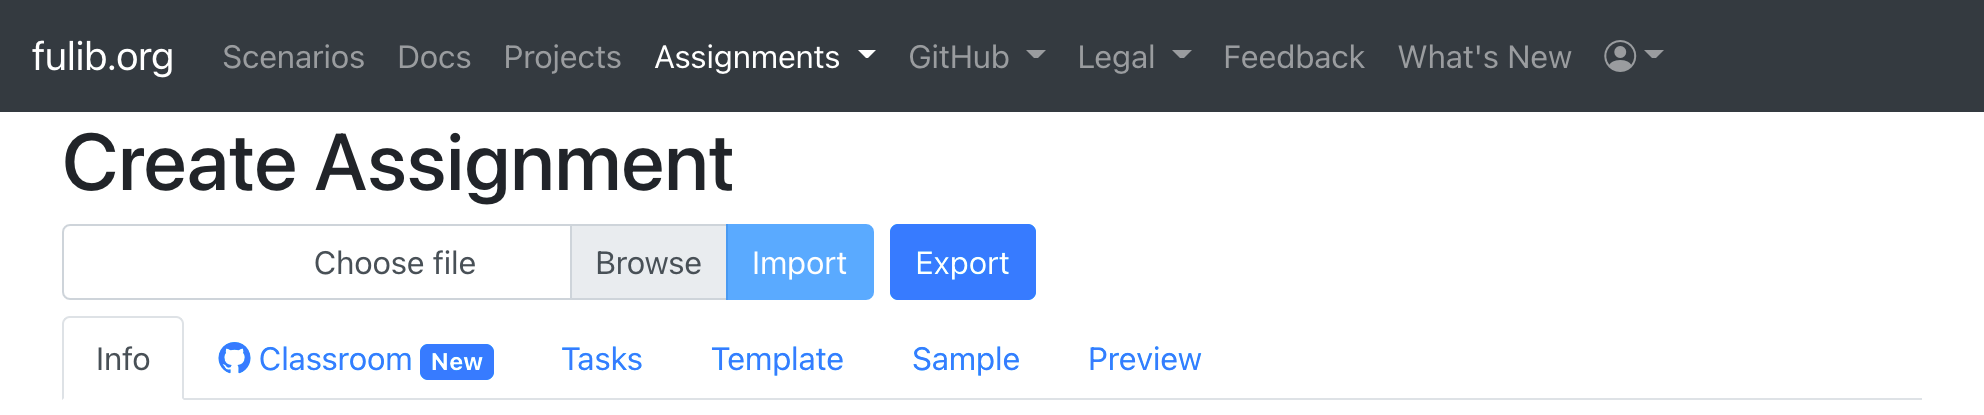
\includegraphics[width=\textwidth]{images/assignment-create-head}
    \caption{Kopf des Formulars zum Erstellen von Assignments}
    \label{fig:assignment-create-head}
\end{figure}

Abbildung~\ref{fig:assignment-create-head} stellt den Kopf des Formulars da, der stets sichtbar ist.
Verschiedene Registerkarten stellen die Aspekte dar, aus denen ein Assignment besteht.
Gleichzeitig ergibt sich aus ihnen eine logische Bearbeitungsreihenfolge der Schritte, in die sich der Erstellungsprozess unterteilt.
Nachfolgend werden einige dieser Aspekte und Schritte beschrieben.

\begin{figure}
    \centering
    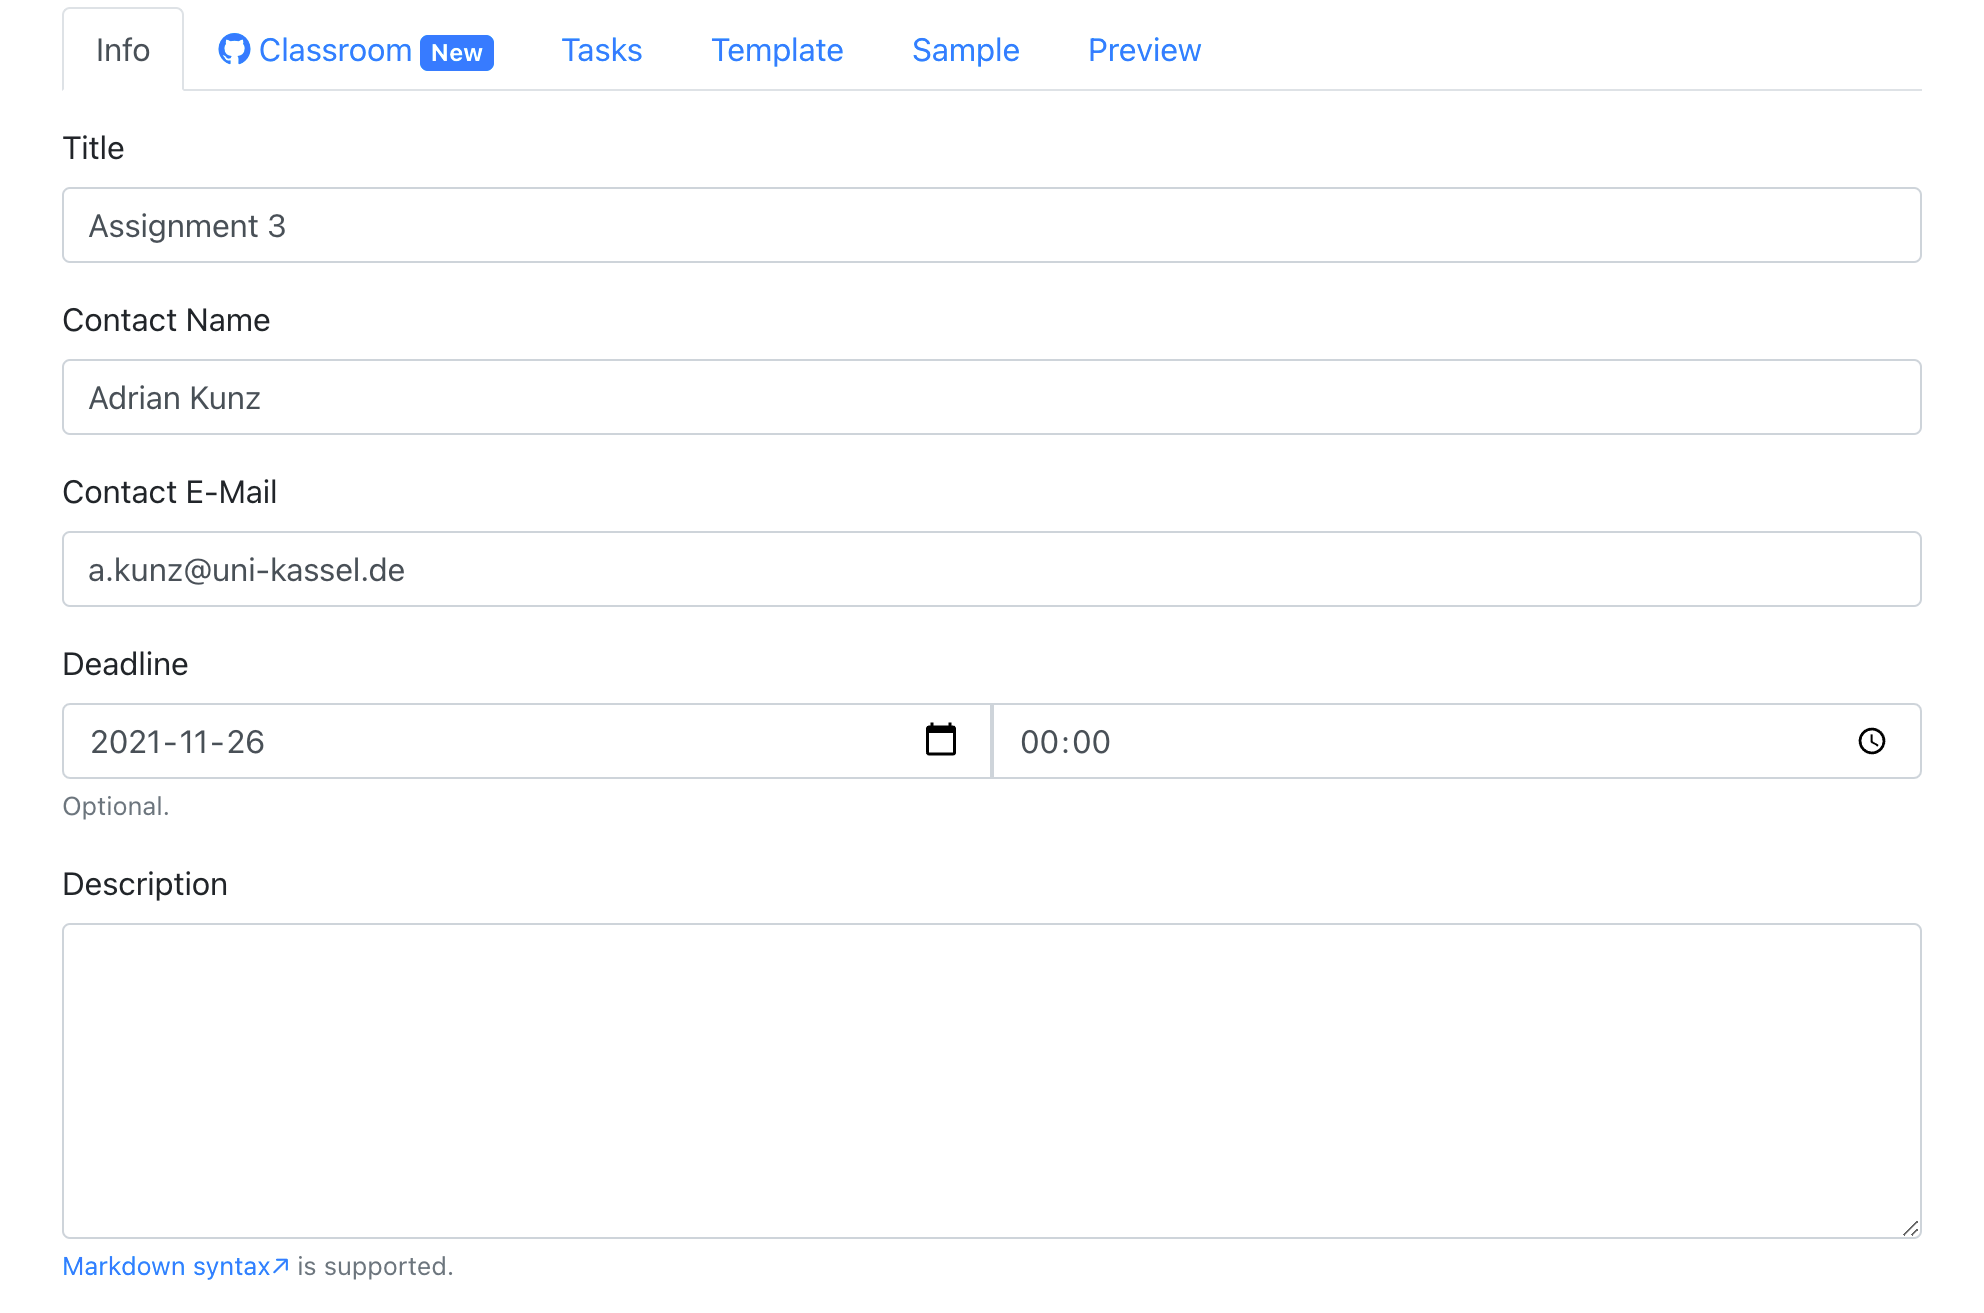
\includegraphics[width=\textwidth]{images/assignment-create-info}
    \caption{Formular für Rahmeninformationen eines Assignments}
    \label{fig:assignment-create-info}
\end{figure}

Zunächst werden einige Rahmeninformationen definiert.
Abbildung~\ref{fig:assignment-create-info} zeigt das zugehörige Formular.
Dazu gehören ein Titel (\textbf{Title}) für das Assignment, welcher der Zuordnung dient.
Ein Ansprechpartner, beispielsweise die Übungsleitung, und dessen Email-Adresse werden in den Feldern \textbf{Contact Name} und \textbf{Contact Email} festgelegt.
Die optionale Abgabefrist (\textbf{Deadline}) hat zwei wesentliche Verwendungszwecke.
Einerseits wird diese für den automatischen Import verwendet, der in Kürze anhand der GitHub Classroom-Integration erläutert wird.
Andererseits kann anhand der Deadline dargestellt werden, welche Lösungen zu spät eingereicht wurden.
Ein Beispiel dafür wird in Abschnitt~\ref{subsec:grading} gezeigt.
Die Beschreibung (\textbf{Description}) kann weitere Informationen über das Assignment enthalten, wird aber nachfolgend nicht verwendet.

\begin{figure}
    \centering
    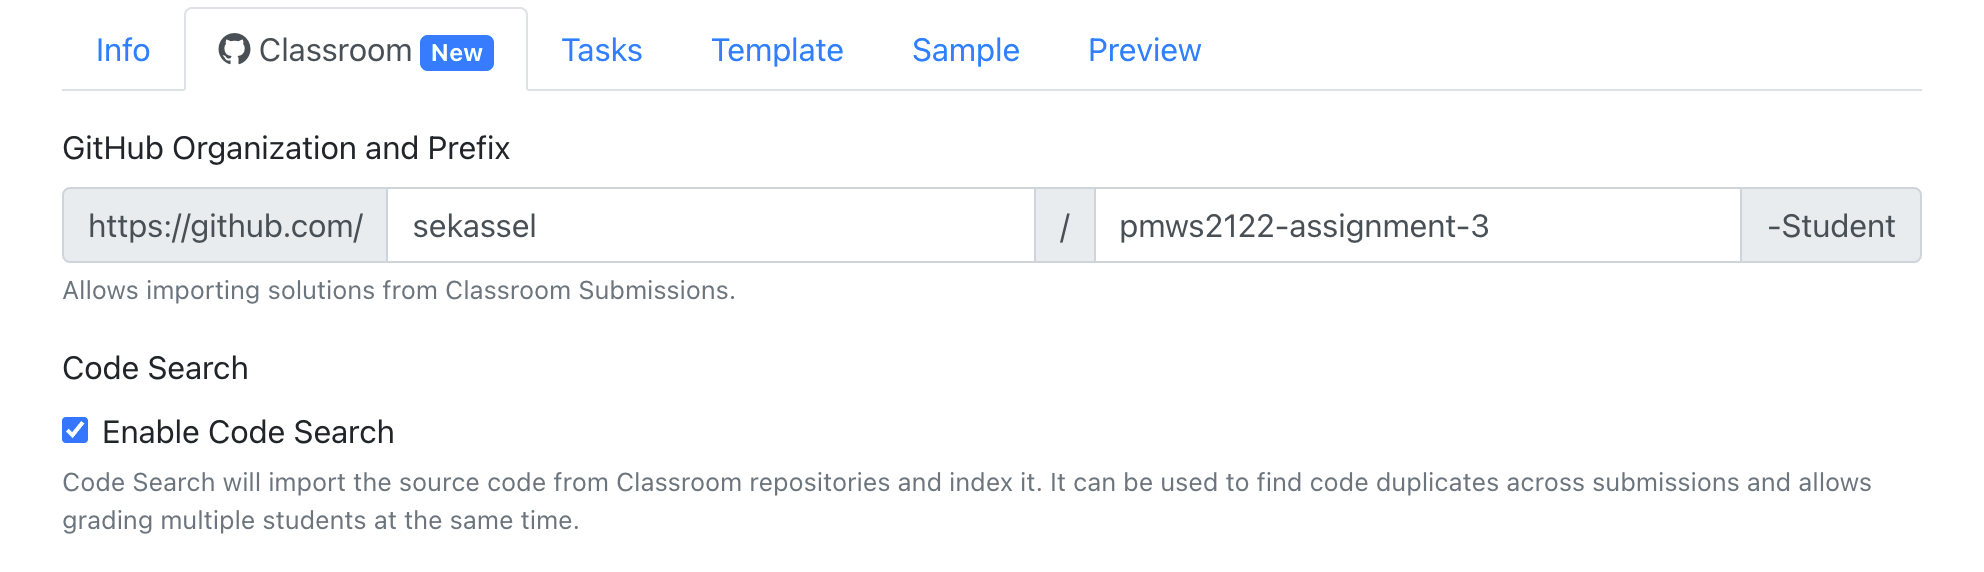
\includegraphics[width=\textwidth]{images/assignment-create-classroom}
    \caption{Formular für GitHub Classroom-Einstellungen eines Assignments}
    \label{fig:assignment-create-classroom}
\end{figure}

Auf der nächsten Seite des Formulars können Angaben für die GitHub Classroom-Integration gemacht werden.
Abbildung~\ref{fig:assignment-create-classroom} zeigt ein Bild dieses Formulars.
Dafür müssen der Name der GitHub-Organisation (\textbf{Organization}) und das Präfix (\textbf{Prefix}) konfiguriert werden.
Dies ermöglicht die manuelle oder zum Zeitpunkt der Deadline automatische Importierung von Lösungen von der Platform.
Anhand der Search-\ac{api} von GitHub\footnote{\url{https://docs.github.com/en/rest/reference/search\#search-repositories}} wird nach allen Repositories in der angegebenen Organisation gesucht, deren Name mit dem Präfix beginnt.
Aus dem Repository-Name ohne Präfix kann der GitHub-Benutzername des Studierenden ermittelt werden, der für die Zuordnung der Lösung verwendet wird.
In Abschnitt~\ref{subsec:grading} ist ein Beispiel für die entstehende Lösungstabelle sichtbar.
Weiterhin wird das neueste Commit zum Zeitpunkt des Imports gespeichert, um die Reproduzierbarkeit einer Bewertung zu gewährleisten.
Insbesondere wird dadurch sichergestellt, dass Studierende ihre Lösungen nicht verfälschen, indem sie Änderungen am Quellcode nach Ablauf der Abgabefrist durchführen oder hochladen.
Anhand des Commits kann der exakte Stand zum Zeitpunkt der Abgabefrist wiederhergestellt werden.
Ist der Haken \textbf{Code Search} gesetzt, werden neben dem Commit auch die Dateien des Repositories heruntergeladen und separat gespeichert.
Diese dienen nicht der Reproduzierbarkeit, sondern der Textsuche, wie in Abschnitt~\ref{subsec:code-search} näher erläutert wird.
Aus diesem Grund wird auch kein Anspruch auf Vollständigkeit der Daten gestellt.
Vergleichsweise große Dateien (> 64KB) werden nicht gespeichert, da gewöhnliche Quellcode-Dateien aus Hausaufgaben-Lösungen diese Größe nicht überschreiten.
\footnote{\todo{Source?}}

\begin{figure}
    \centering
    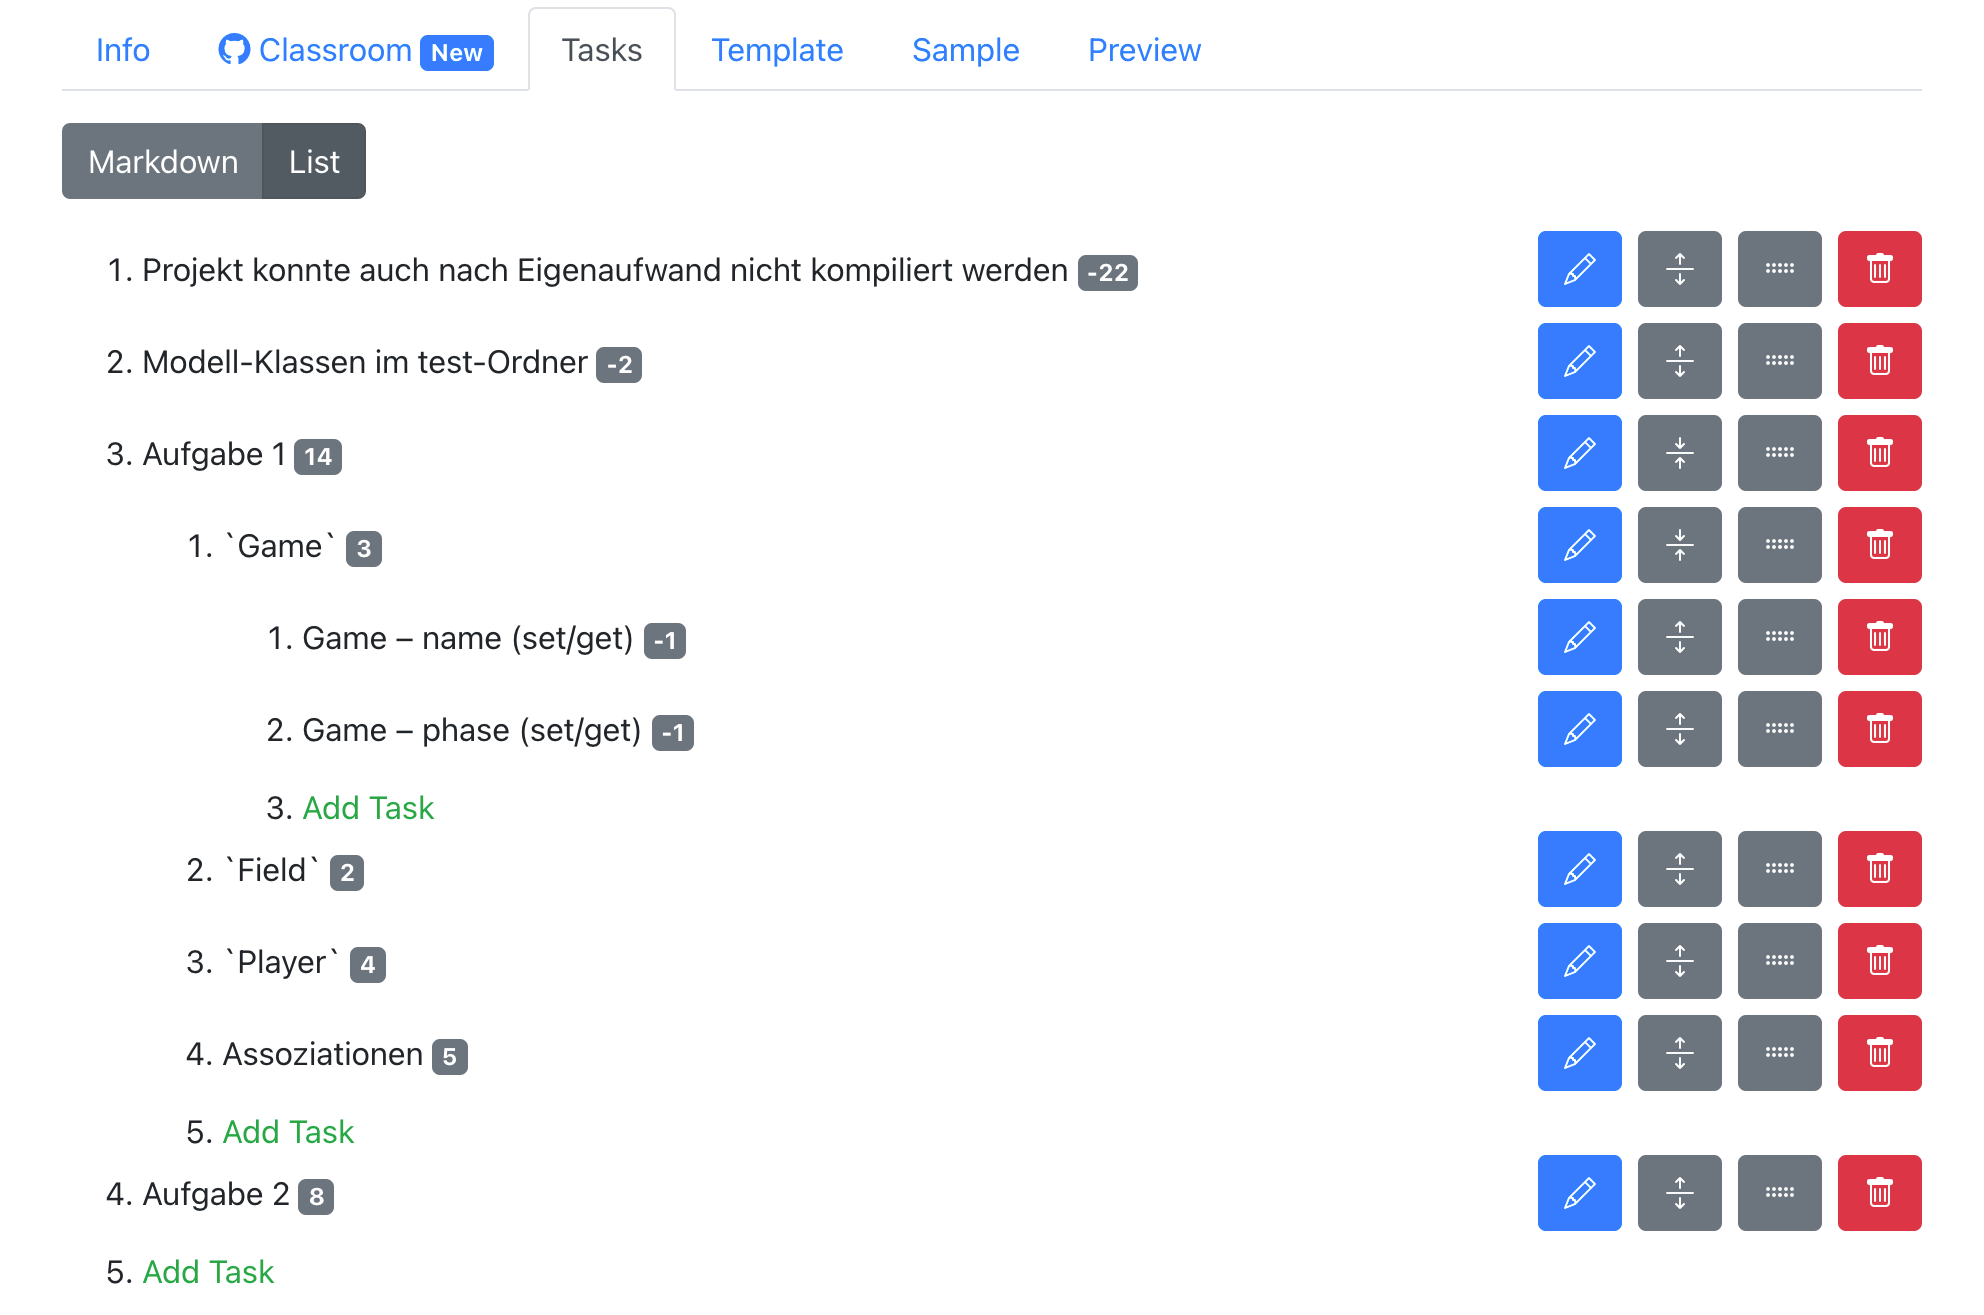
\includegraphics[width=\textwidth]{images/assignment-create-tasks-list}
    \caption{Baum-Editor für Teilaufgaben}
    \label{fig:assignment-create-tasks-list}
\end{figure}

Nun muss die Struktur des Aufgabenblatts anhand von Teilaufgaben, genannt Tasks, definiert werden.
Diese können beliebig geschachtelt und angeordnet werden, weshalb ein spezieller Editor für die Bearbeitung notwendig ist.
Abbildung~\ref{fig:assignment-create-tasks-list} zeigt, wie dieser in der Oberfläche aussieht.
Jeder Task besteht mindestens aus einer kurzen Beschreibung, die auch als Titel dienen kann, und einer Punktzahl.
In der Abbildung ist bereits erkennbar, dass eine Punktzahl nicht zwangsweise positiv sein muss.
Ein Task mit negativer Punktzahl wird als Abzug bezeichnet und kann besonders dann eingesetzt werden, wenn eine Aufgabe aus vielen ungeordneten Teilen besteht.
Dann ist es möglich, in einem Feedback nur die zutreffenden Abzüge darzustellen und damit die Übersichtlichkeit und Nachvollziehbarkeit zu verbessern.

Neben jedem Task werden vier Buttons angezeigt.
Der blaue Stift öffnet die Detailansicht des Tasks, die in den Abbildungen~\ref{fig:assignment-create-tasks-detail} dargestellt ist und im Folgenden beschrieben wird.
Mit dem Pfeile-Button kann ein Task aus- oder eingeklappt werden, um die Untertasks anzuzeigen oder zu verbergen.
Die nächste Schaltfläche kann verwendet werden, um die Reihenfolge der Tasks anzupassen oder Tasks unter andere zu verschieben.
Zuletzt erlaubt der Mülleimer-Button das Löschen eines Tasks.
Dabei handelt es sich nicht um eine sofortige Löschung, der Task wird lediglich als gelöscht markiert und kann wiederhergestellt werden, um eventuellen Datenverlust zu vermeiden.

\begin{figure}
    \centering
    \begin{subfigure}[t]{0.475\textwidth}
        \centering
        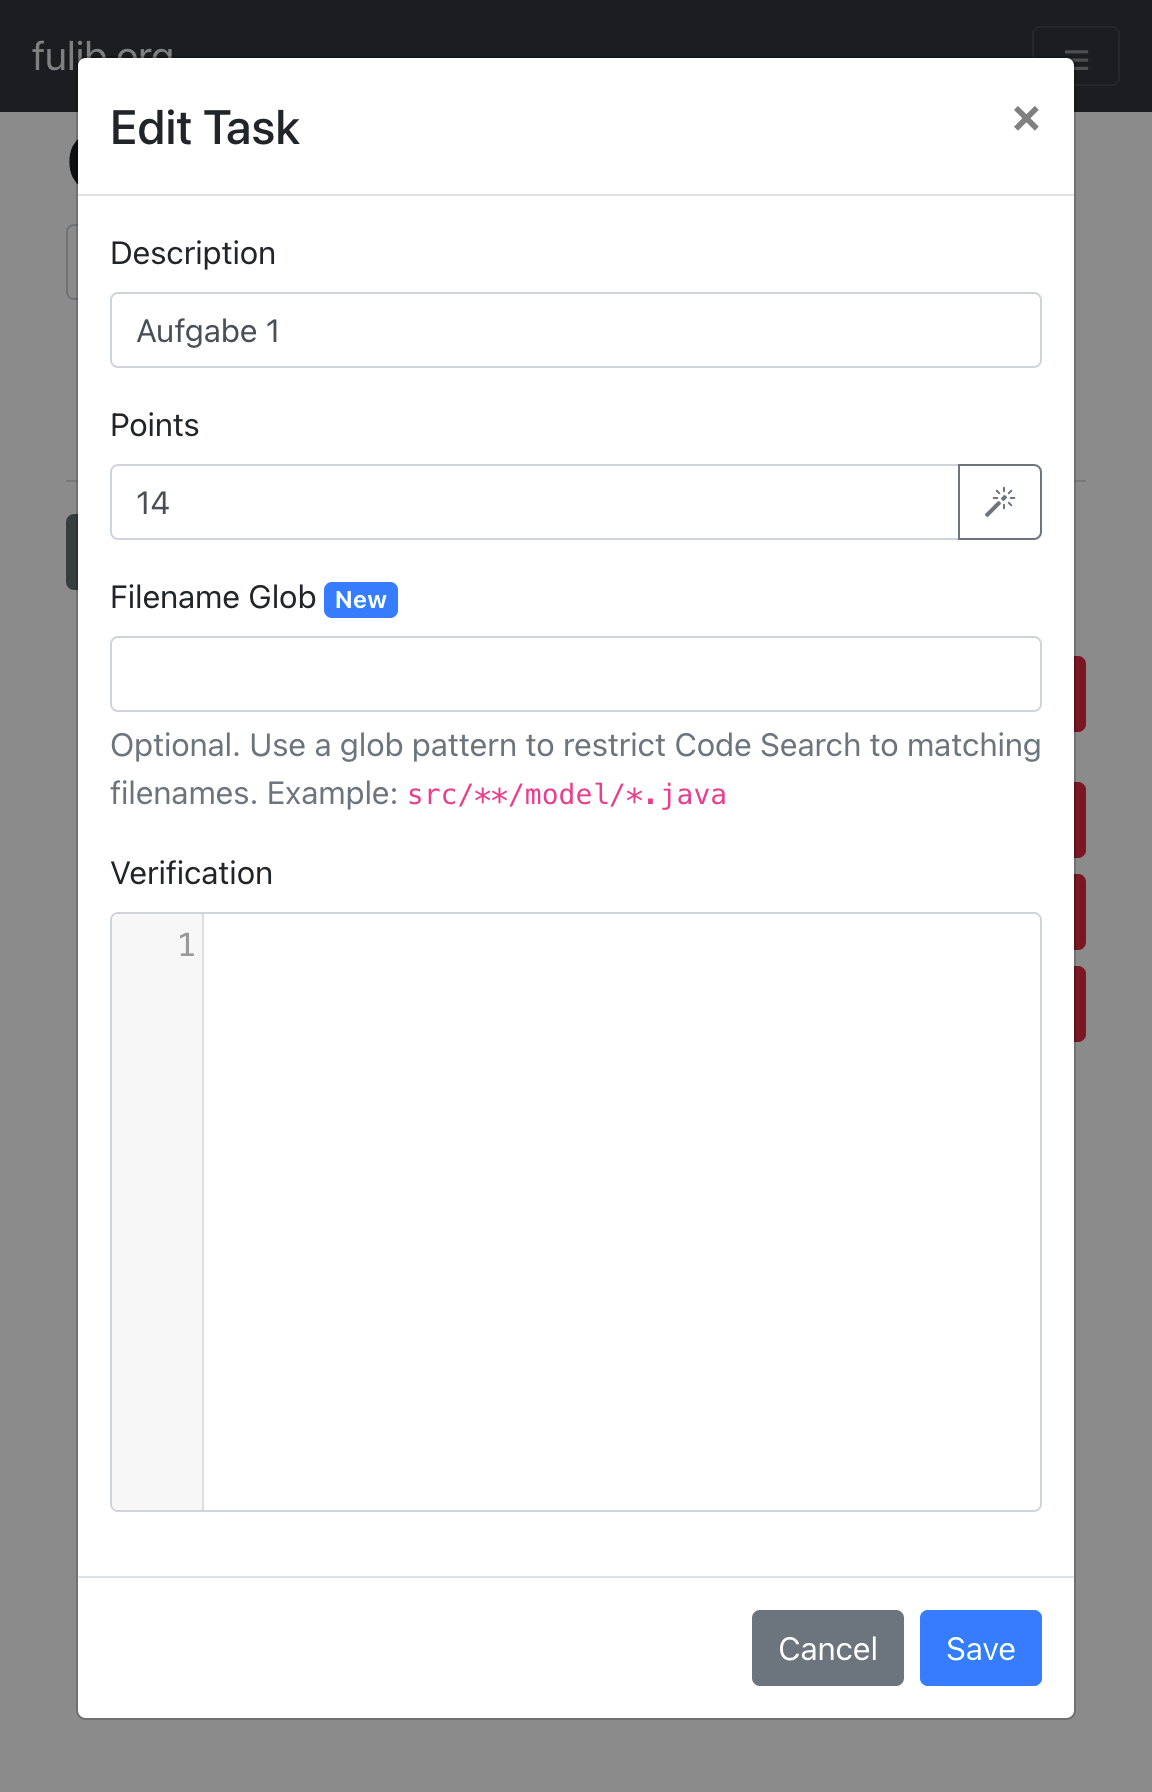
\includegraphics[width=\textwidth]{images/assignment-create-tasks-detail-1}
        \caption{Detailansicht eines positiven Tasks mit Untertasks}
        \label{fig:assignment-create-tasks-detail-1}
    \end{subfigure}
    \hfill
    \begin{subfigure}[t]{0.475\textwidth}
        \centering
        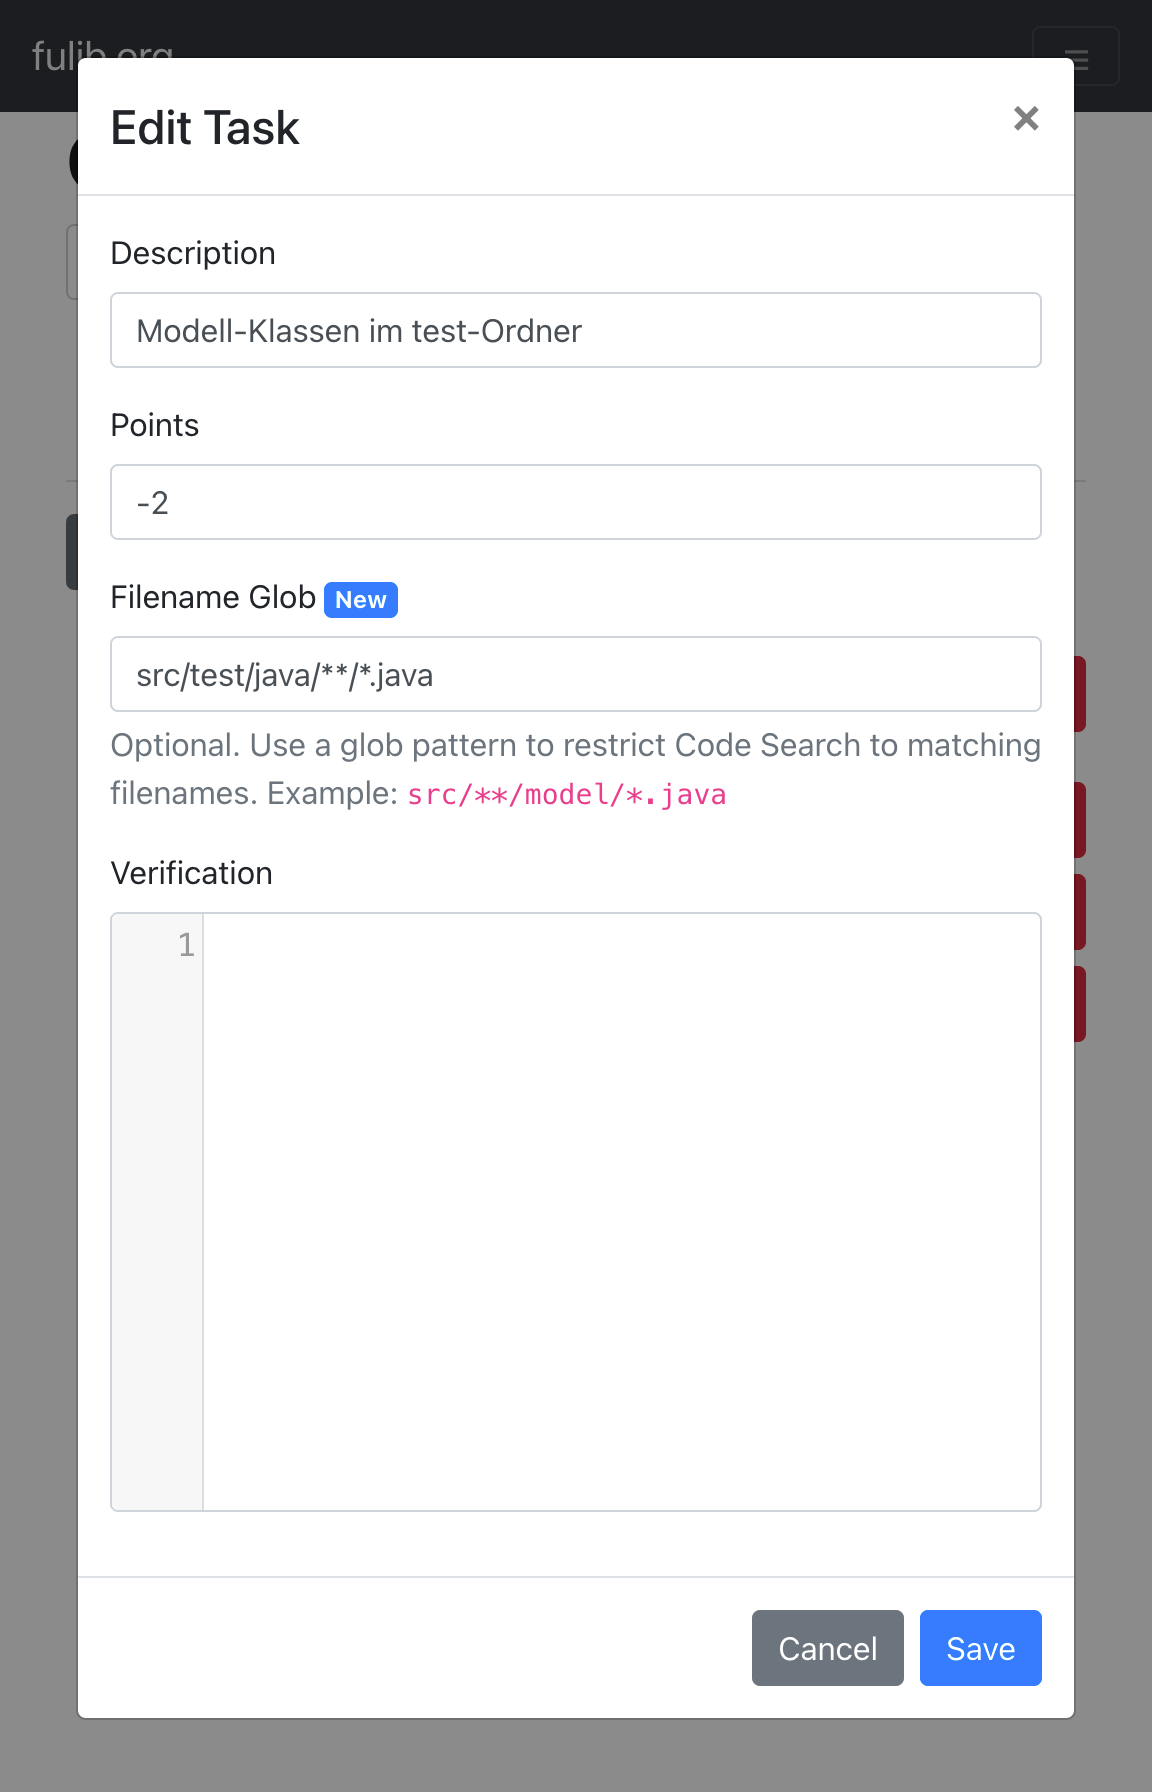
\includegraphics[width=\textwidth]{images/assignment-create-tasks-detail-2}
        \caption{Detailansicht eines negativen Tasks}
        \label{fig:assignment-create-tasks-detail-2}
    \end{subfigure}
    \caption{Detailansicht zweier Tasks}
    \label{fig:assignment-create-tasks-detail}
\end{figure}

\todo{
    Teilaufgaben, Punkteberechnung.
    GitHub Classroom Import.
}

\subsection{Bewertung}\label{subsec:grading}

\todo{
    Sharing.
    QoL in Tabelle.
    Oberfläche für Evaluation und Snippets.
    Feedback mit GitHub Classroom, Email, etc.
}

\subsection{Statistiken}\label{subsec:statistics}

\todo{
    Evaluations als Darstellung der Code Search-Effektivität.
    Task-Liste als Information über schwierigste Teilaufgaben / Problemquellen.
}

\subsection{Code Search}\label{subsec:code-search}

\todo{
    Code Search als Anwendung von Elasticsearch.
}

\section{fulibFeedback}\label{sec:fulibFeedback}

\subsection{VSCode Extension}\label{subsec:vscode-extension}

\todo{
    Einfacher Client für Language Server.
    Einstellungen.
    Protocol Handler für Konfiguration.
}

\subsection{Language Server}\label{subsec:language-server}

\todo{
    Selection und Diagnostics.
    Wiederverwendbar für andere IDEs.
}
